\section{基本介绍(重要)}

如果您先前已经在使用旧版本集成工具,只是想迁移至新版本,则请移步\nameref{how_to_update}。

本节简述本集成工具的使用方法及注意事项。\textbf{\color{red} 阅读本文档时,如图片尺寸过小,可以通过您使用的 PDF 阅读器(浏览器或专业 PDF 编辑软件)自带的放大/缩小功能查看本文档中的图片。}

\begin{figure}[H]
    \Centering
    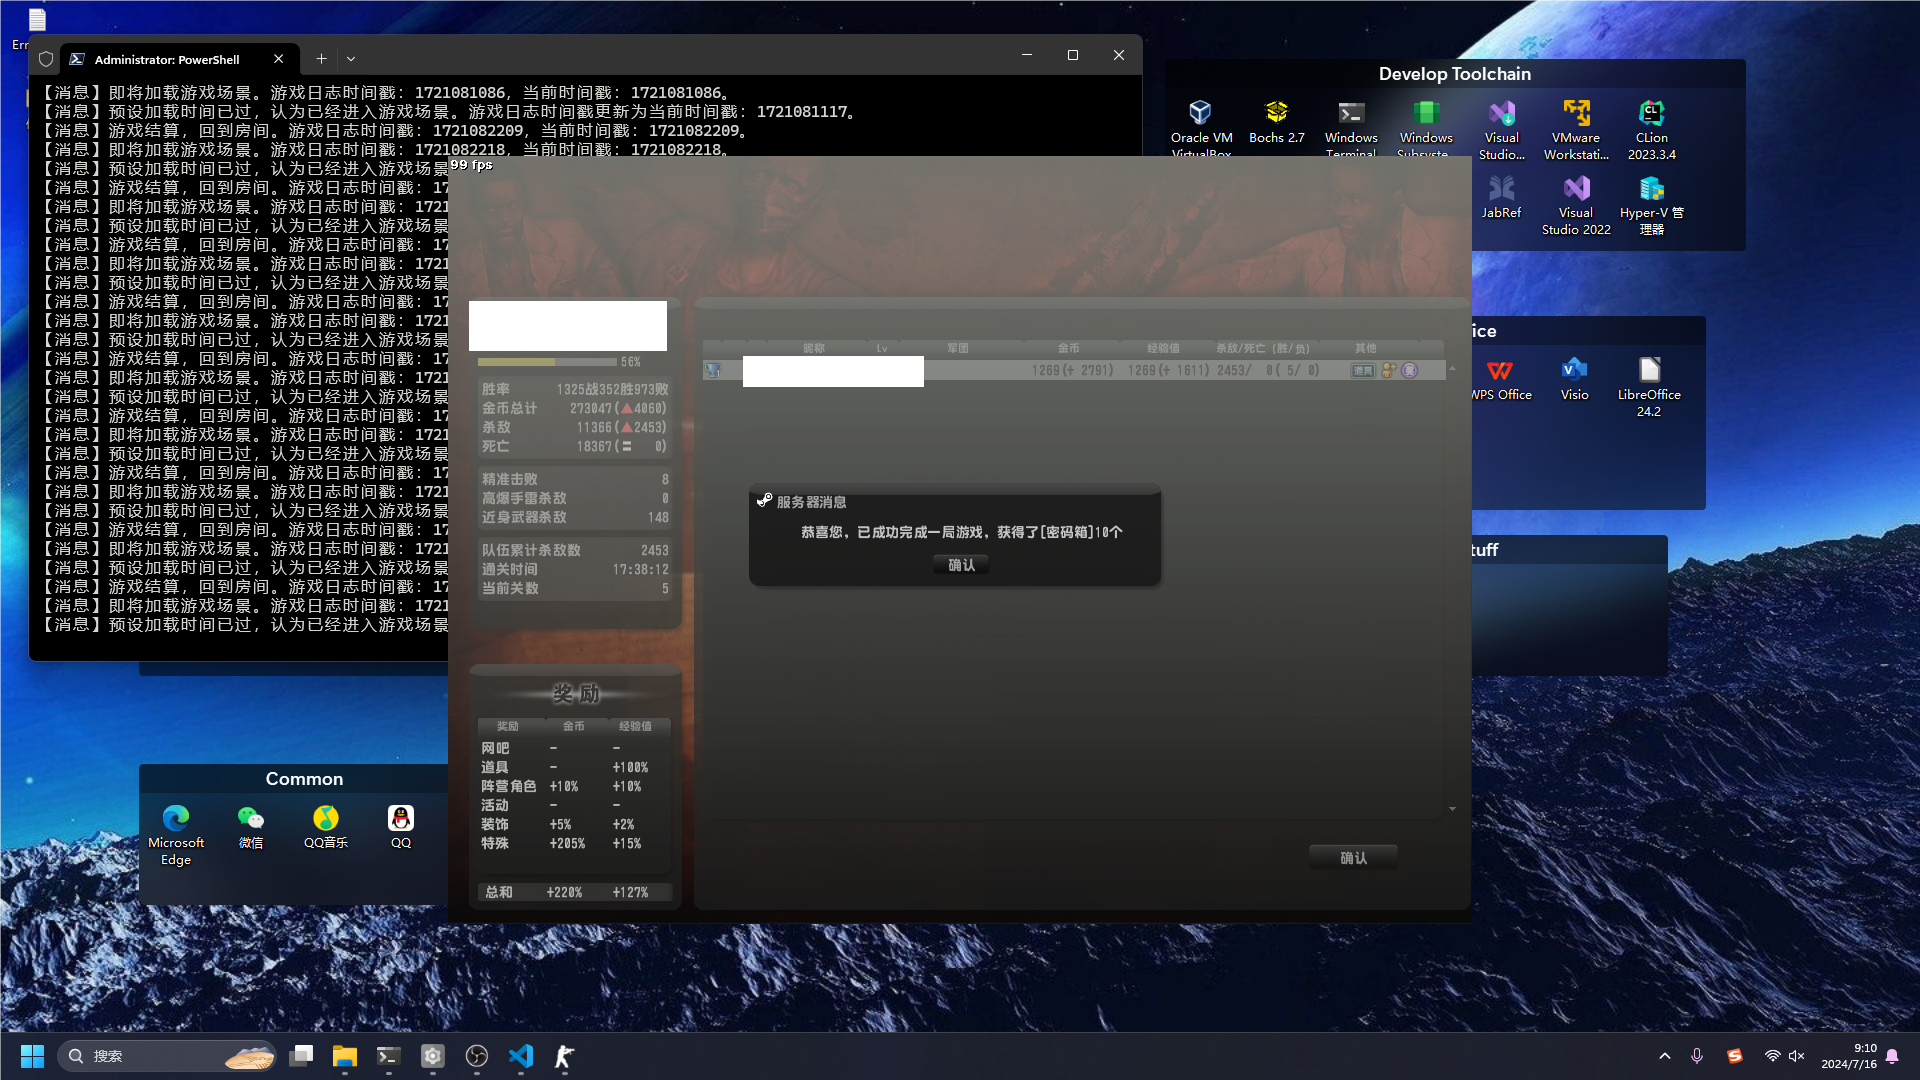
\includegraphics[width=\textwidth]{assets/intro/controller.png}
    \caption{运行效果展示}
\end{figure}

\subsection{开始之前}

\textbf{\color{red}Windows 会锁定从网络上下载得到的文件,需先对其解除锁定,操作步骤如下:}

\begin{figure}[H]
    \Centering
    \parbox[l]{\textwidth}{对下载得到的压缩包右键并点击“属性”(图 \ref{ch0fig-unlock-0})。}
    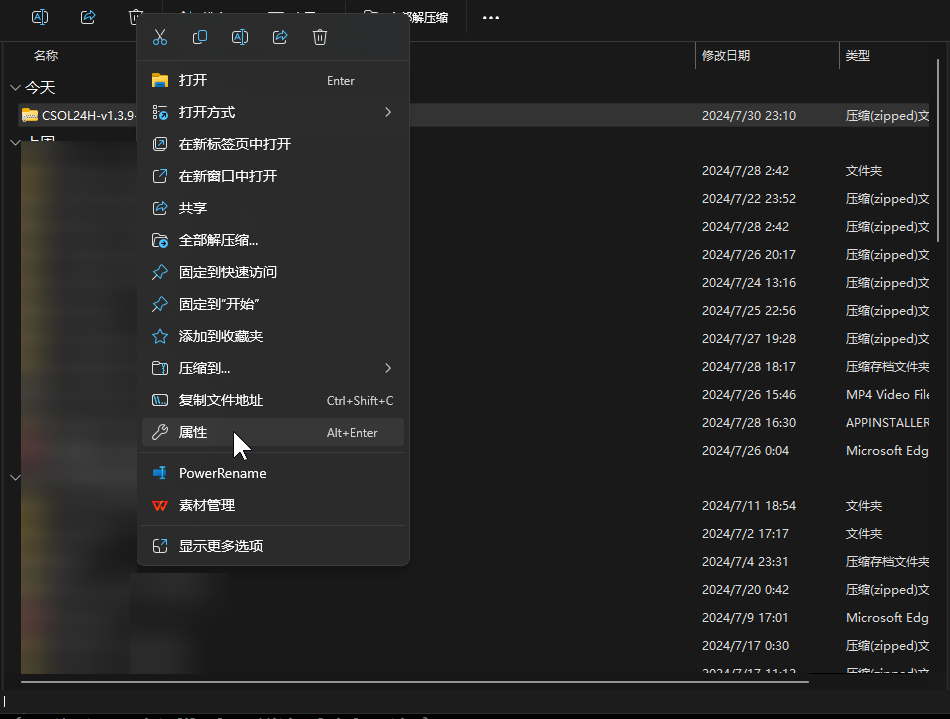
\includegraphics[width=\textwidth]{assets/intro/unlock_00.png}
    \caption{右键后在弹框中点击“属性”}
    \label{ch0fig-unlock-0}
\end{figure}

\begin{figure}[H]
    \Centering
    \parbox[l]{\textwidth}{点击“解除锁定”(图 \ref{ch0fig-unlock-1})。如果压缩包未被锁定(没有“解除锁定”选项),可忽略此步骤。}
    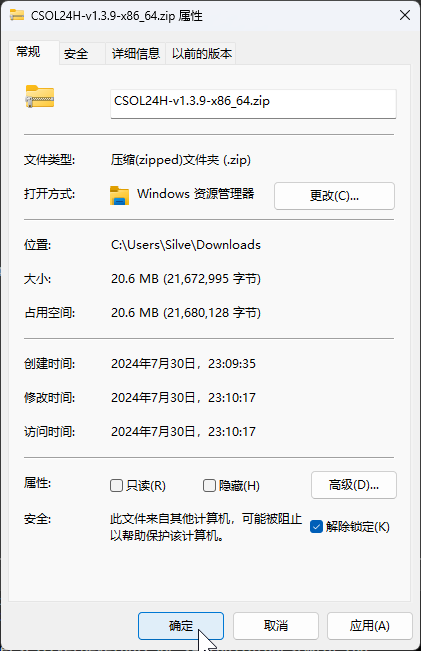
\includegraphics[width=\textwidth]{assets/intro/unlock_01.png}
    \caption{点击“解除锁定”并确认}
    \label{ch0fig-unlock-1}
\end{figure}

将解除锁定后的压缩包解压,\textbf{\color{red}解压路径不能包含非英文字符}。
Windows 文件系统不区分文件名的大小写。因此,若您在接下来的步骤中遇到名称相同但大小写不同的文件名,应将其视为完全一样的文件名。

% Windows 默认情况下严格阻止运行任何 Powershell 脚本文件(后缀为 \lstinline{.ps1}),因此若您是第一次使用本工具,需要做如下配置。

% 对于 Windows 11 23H2 及以上版本的用户修改较为简单:打开“设置”,点击“系统”→“开发者选项”(图 \ref{ch0fig-win11-23h2-0}),在“Powershell”下拉选项中打开图示选项即可(图 \ref{ch0fig-win11-23h2-1})。下面针对 Windows 11 23H2 以下版本用户的设置步骤可忽略。

% \begin{figure}[H]
%     \Centering
%     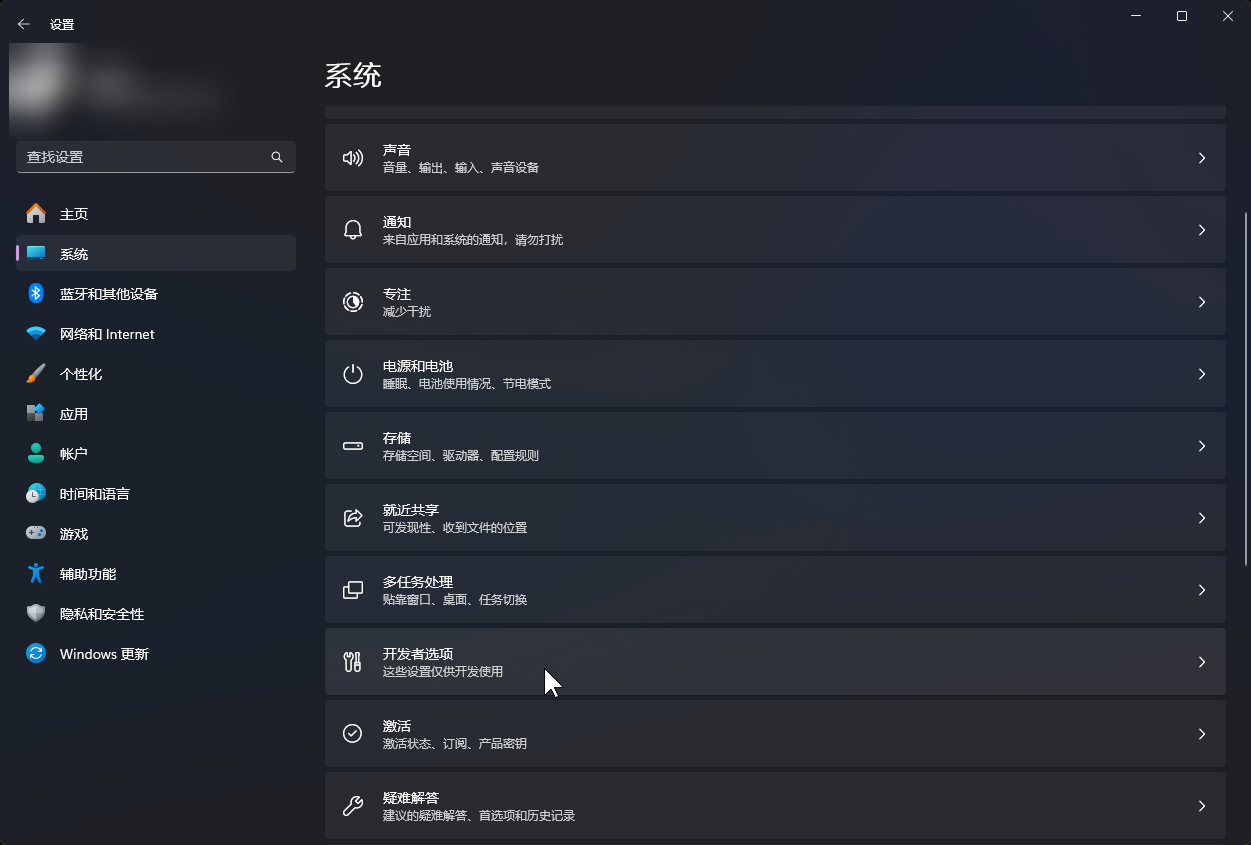
\includegraphics[width=\textwidth]{assets/intro/win11_23h2_00.png}
%     \caption{点击“开发者选项”}
%     \label{ch0fig-win11-23h2-0}
% \end{figure}

% \begin{figure}[H]
%     \Centering
%     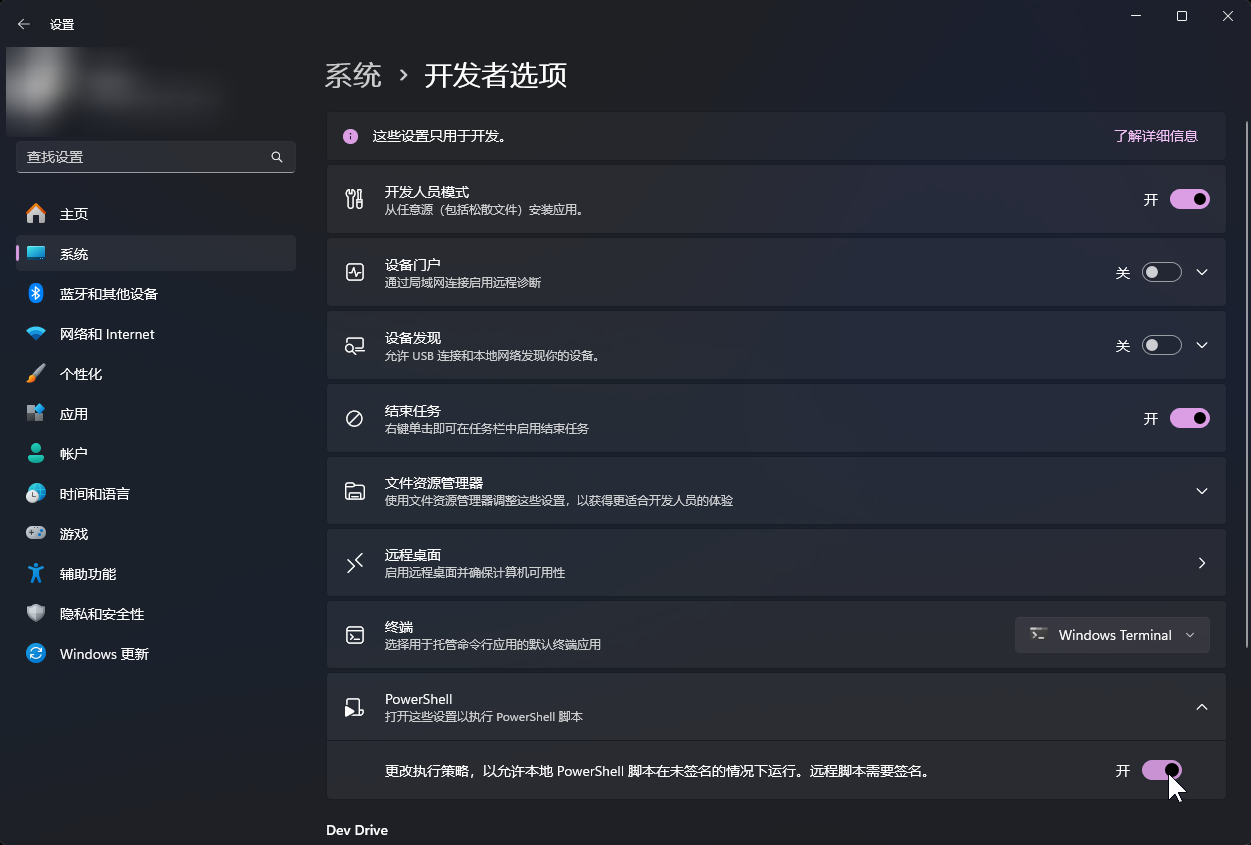
\includegraphics[width=\textwidth]{assets/intro/win11_23h2_01.png}
%     \caption{修改执行策略}
%     \label{ch0fig-win11-23h2-1}
% \end{figure}

% 对于 Windows 11 23H2 以下版本的用户,需按照以下步骤操作:

% 按下 \lstinline{Win} \lstinline{R},输入 \lstinline{powershell}。然后,\textbf{\color{red}按下 \lstinline{Ctrl} \lstinline{Shift} \lstinline{Enter} 以管理员权限打开 Powershell 窗口}(图 \ref{ch0fig-run-pwsh-as-admin})。

% \begin{figure}[H]
%     \Centering
%     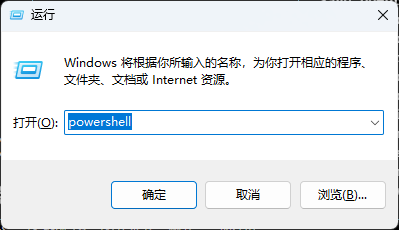
\includegraphics[width=\textwidth]{assets/intro/run_pwsh_as_admin.png}
%     \caption{在“运行”中输入 \lstinline{powershell},并按 \lstinline{Ctrl} \lstinline{Shift} \lstinline{Enter}}
%     \label{ch0fig-run-pwsh-as-admin}
% \end{figure}

% 在 Powershell 窗口输入下面的命令:

% \begin{minted}{powershell}
% Set-ExecutionPolicy -Scope CurrentUser -ExecutionPolicy RemoteSigned
% \end{minted}

% 回车运行上述命令(图 \ref{ch0fig-change-execution-policy}),过程中可能需要您输入“Y”确认(图 \ref{ch0fig-confirm-execution-policy})。运行完成后即可关闭窗口。

% \begin{figure}[H]
%     \Centering
%     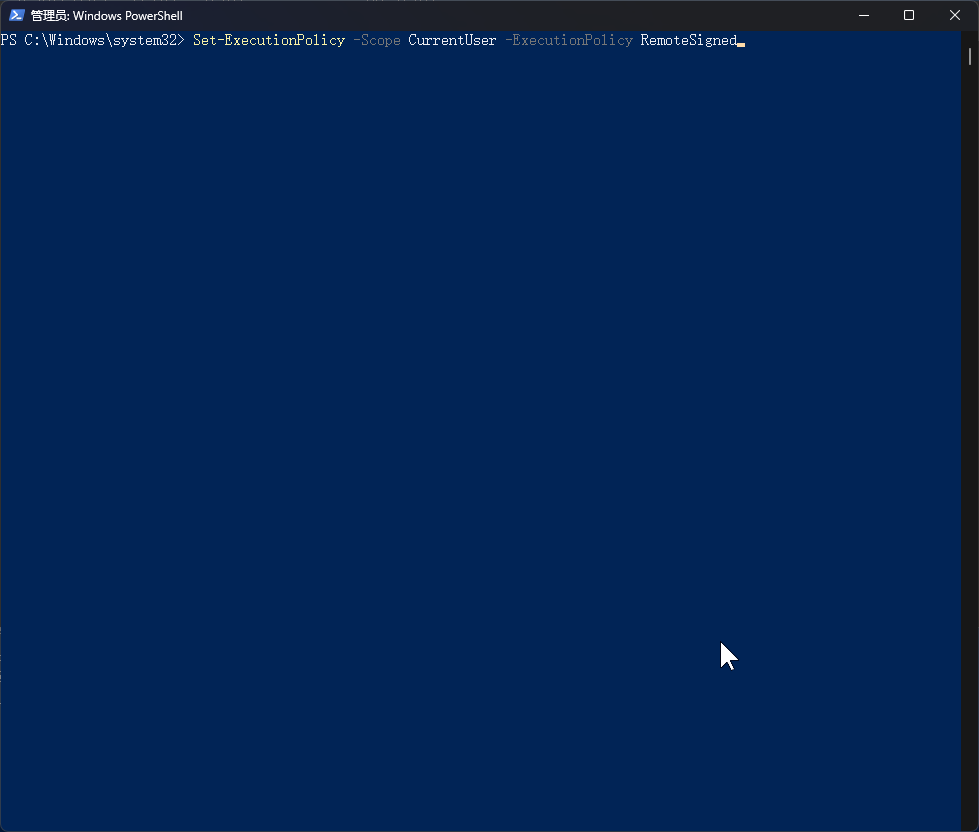
\includegraphics[width=\textwidth]{assets/intro/confirm_execution_policy_00.png}
%     \caption{键入修改执行策略的命令}
%     \label{ch0fig-change-execution-policy}
% \end{figure}

% \begin{figure}[H]
%     \Centering
%     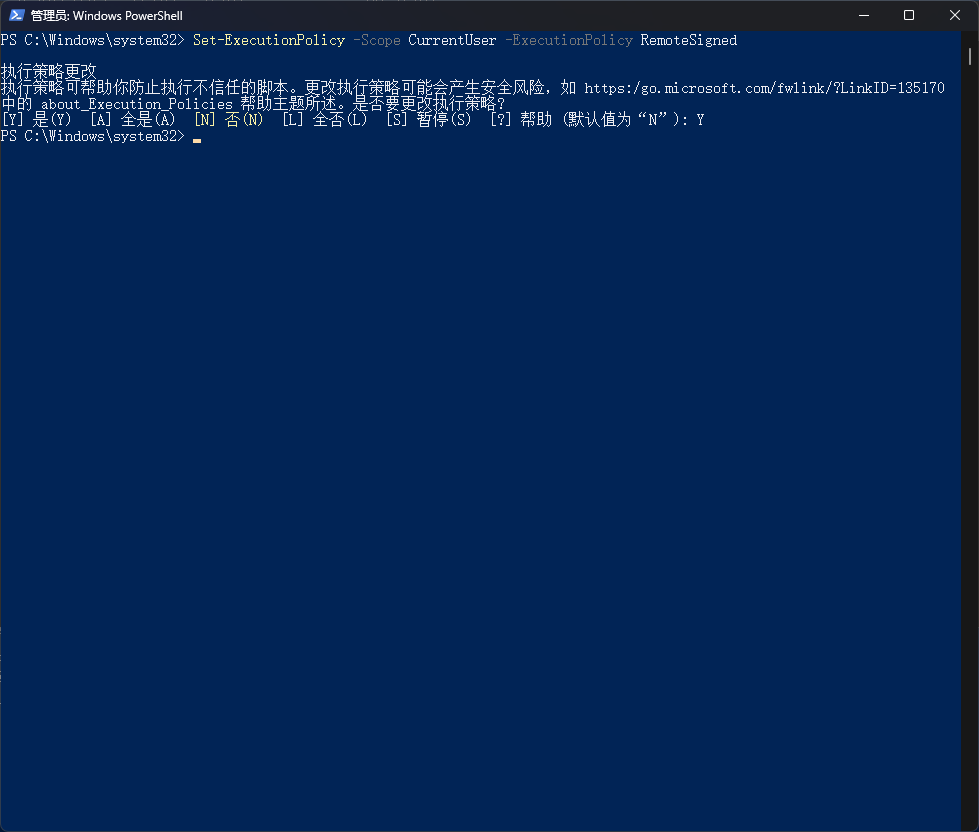
\includegraphics[width=\textwidth]{assets/intro/confirm_execution_policy_01.png}
%     \caption{确认修改执行策略}
%     \label{ch0fig-confirm-execution-policy}
% \end{figure}
% 
\subsection{罗技软件导入 Lua \lstinline{Executor}(执行器) 模块}

双击运行集成工具文件夹中的 \lstinline{Install.cmd},点击在 Powershell 中运行(图 \ref{ch0fig-run-install-script}),您会看到在目录中生成了一个新文件 \lstinline{Executor.lua}(如果已经存在此文件,则会生成新的文件并覆盖它),如果没有看到,请刷新一下文件管理器页面。
\textbf{\color{red} 如果变动了安装路径(如:移动集成工具文件夹位置、将集成工具文件夹重命名),则需要重新运行一次 \lstinline{Install.cmd},并重新在 Logitech G Hub 中导入并执行“保存并运行”操作(详见下文)。}

\begin{figure}[H]
    \Centering
    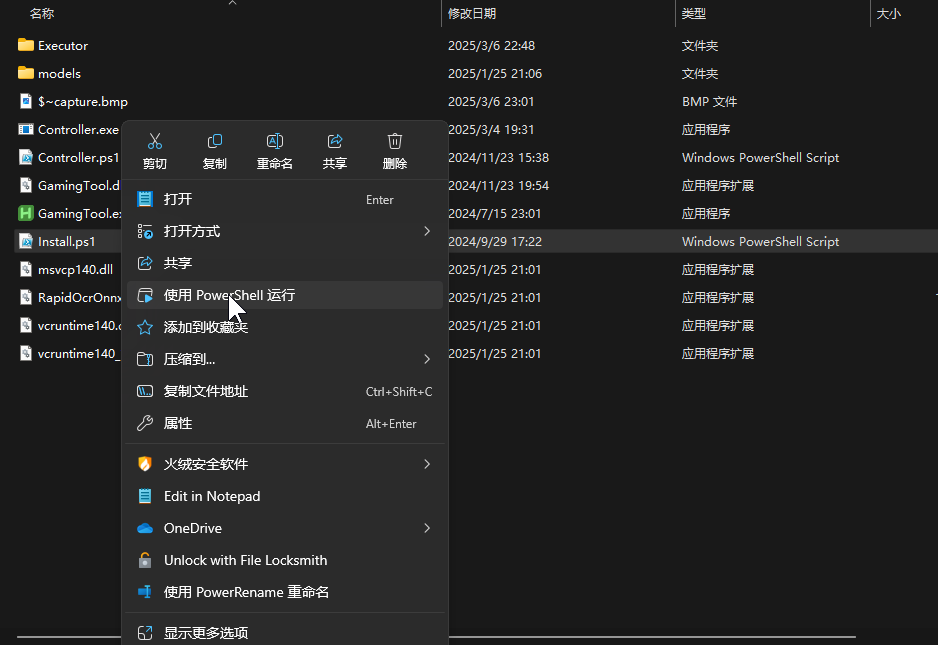
\includegraphics[width=\textwidth]{assets/intro/install.png}
    \caption{运行 \lstinline{Install.cmd}}
    \label{ch0fig-run-install-script}
\end{figure}

\begin{figure}[H]
    \Centering
    \parbox[l]{\textwidth}{前往罗技官网下载安装最新版的 Logitech G Hub 软件(图 \ref{ch0fig-download-lghub},以下简称为“罗技软件”)。\textbf{\color{red}本集成工具并不需要您拥有任何的罗技硬件设备。}}
    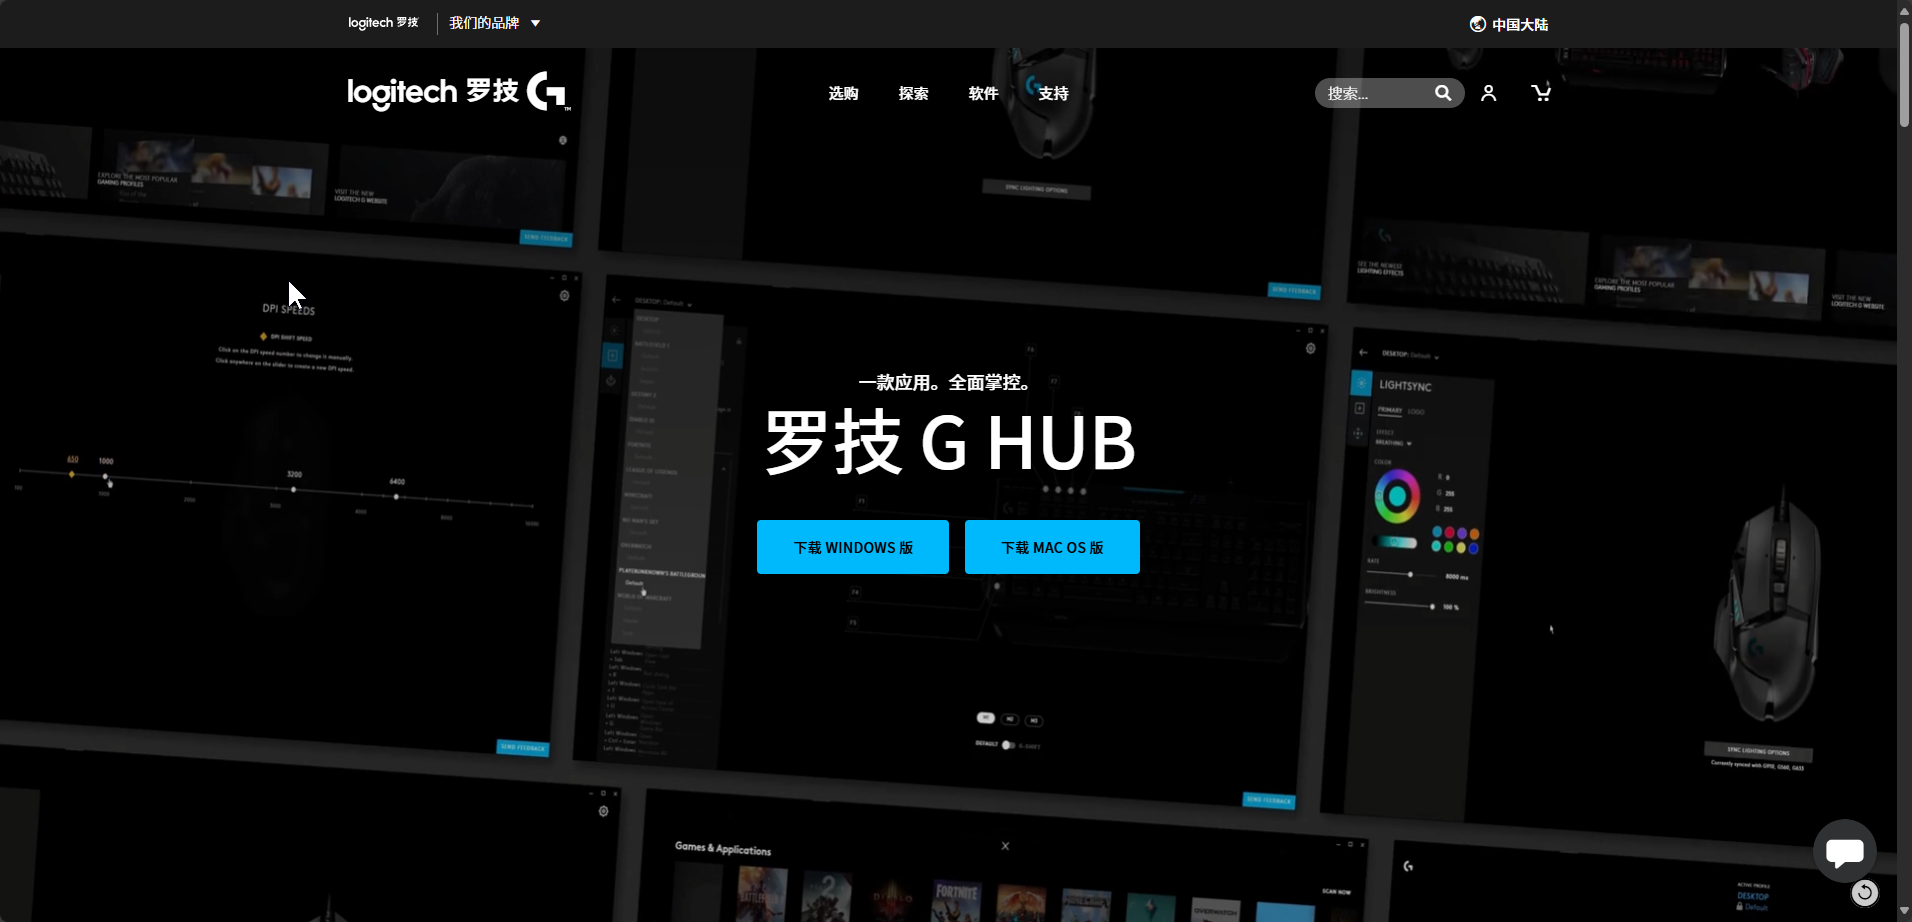
\includegraphics[width=\textwidth]{assets/intro/download-lghub.png}
    \caption{从官网下载最新版 Logitech G Hub}
    \label{ch0fig-download-lghub}
\end{figure}

\begin{figure}[H]
    \Centering
    \parbox[l]{\textwidth}{随后,安装并\textbf{\color{red}以管理员权限}启动 Logitech G Hub 软件。否则会因为权限问题导致游戏无法正确接收软件发出的键鼠消息。}
    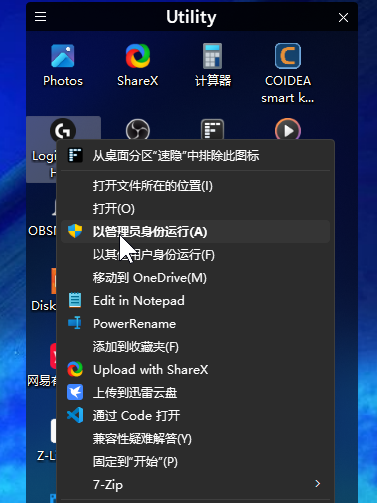
\includegraphics[width=\textwidth]{assets/intro/run_lghub.png}
    \caption{以管理员权限运行 Logitech G Hub}
\end{figure}

如果您之前已经安装运行过罗技软件,或者安装罗技软件后自动运行,则需要注意:当已经存在罗技软件进程正在运行时,运行罗技软件不会再启动新的实例,新打开的进程将会退出以保留旧进程。
\textbf{\color{red}因此,当存在正以普通权限运行的罗技软件进程时,以管理员权限启动罗技软件是无效的。故在以管理员权限启动罗技软件前,请务必确保罗技软件相关进程处于关闭状态。}

\begin{figure}[H]
    \Centering
    \parbox[l]{\textwidth}{确认 Logitech G Hub 是否正在运行的方法为:打开任务管理器,搜索“logi”(图 \ref{ch0fig-search-lghub-process})。}
    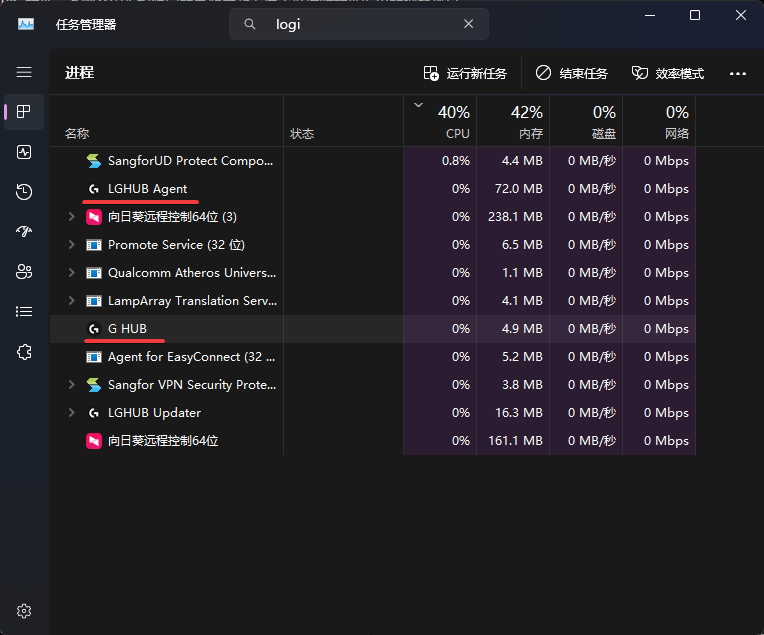
\includegraphics[width=\textwidth]{assets/intro/search_lghub_process.png}
    \caption{搜索罗技软件进程}
    \label{ch0fig-search-lghub-process}
\end{figure}

\begin{figure}[H]
    \Centering
    \parbox[l]{\textwidth}{如果存在正在运行的 Logitech G Hub 进程,则结束\textbf{\color{red}除“Logitech Updater”(罗技软件更新守护进程,无需关闭)}以外的所有与罗技软件相关的进程(图 \ref{ch0fig-terminate-lghub-0}、\ref{ch0fig-terminate-lghub-1})。}
    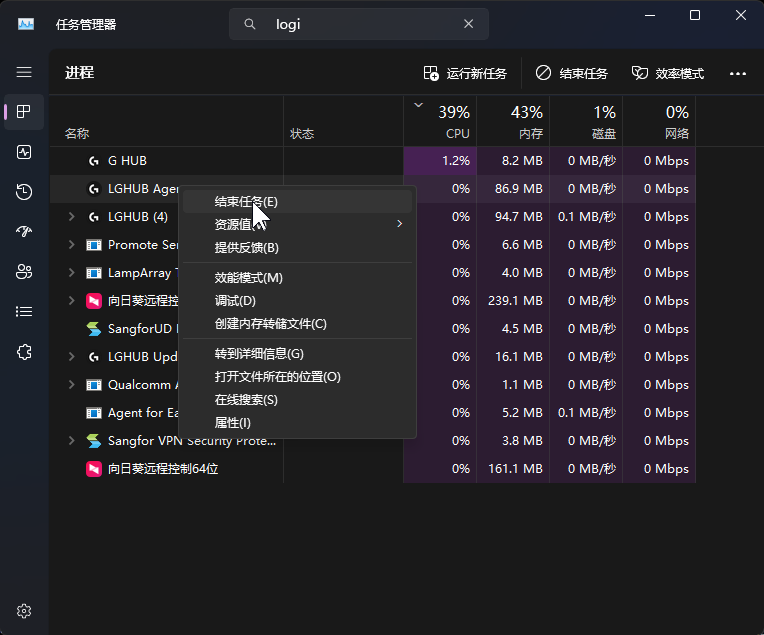
\includegraphics[width=\textwidth]{assets/intro/terminate_lghub_00.png}
    \caption{结束罗技软件进程 - 1}
    \label{ch0fig-terminate-lghub-0}
    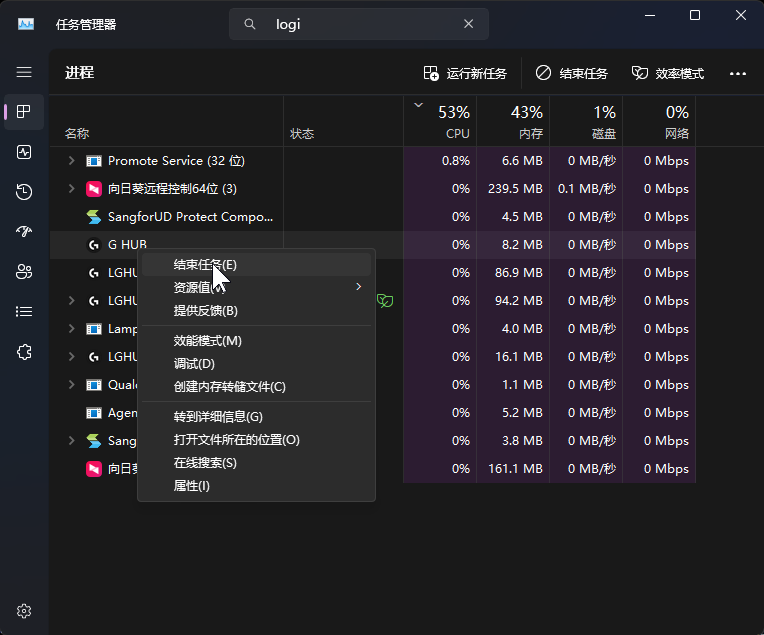
\includegraphics[width=\textwidth]{assets/intro/terminate_lghub_01.png}
    \caption{结束罗技软件进程 - 2}
    \label{ch0fig-terminate-lghub-1}
\end{figure}

\begin{figure}[H]
    \Centering
    \parbox[l]{\textwidth}{上述操作完成后,以管理员权限打开罗技软件,进入罗技软件主界面(图 \ref{ch0fig-lghub})。}
    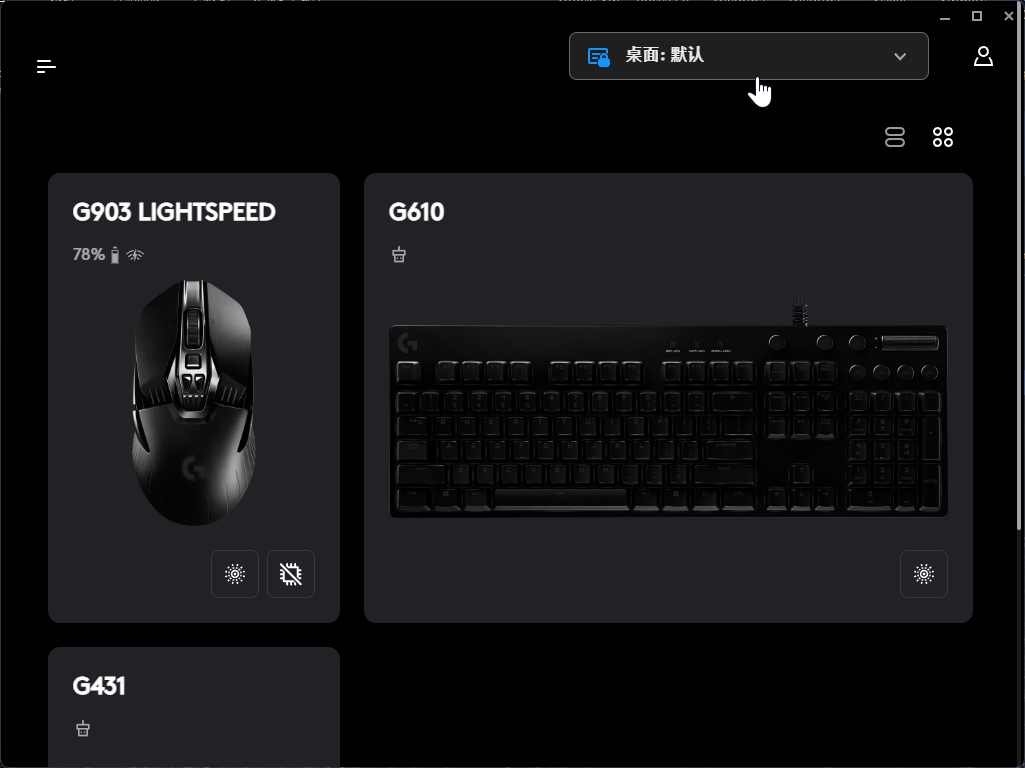
\includegraphics[width=\textwidth]{assets/intro/lghub.png}
    \caption{罗技软件主界面}
    \label{ch0fig-lghub}
\end{figure}

\begin{figure}[H]
    \Centering
    \parbox[l]{\textwidth}{点击左上角展开菜单(图 \ref{ch0fig-lghub-menu})。}
    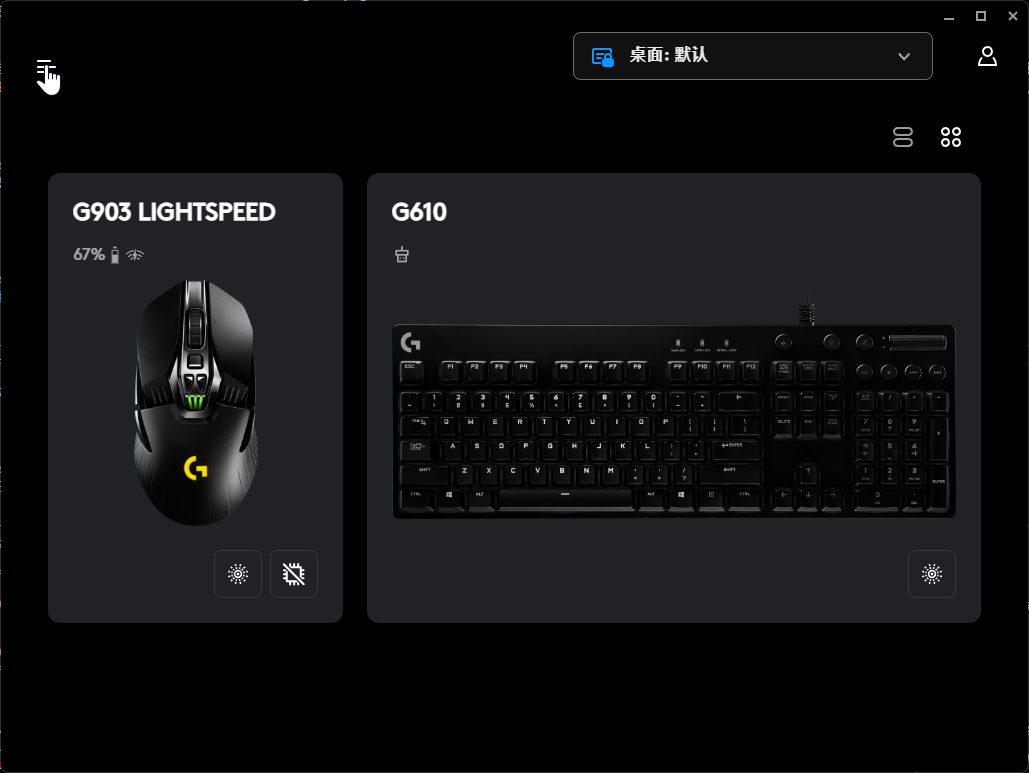
\includegraphics[width=\textwidth]{assets/intro/lghub_menu.png}
    \caption{展开左上角菜单}
    \label{ch0fig-lghub-menu}
\end{figure}

\begin{figure}[H]
    \Centering
    \parbox[l]{\textwidth}{点击“设置”(图 \ref{ch0fig-lghub-setting})。}
    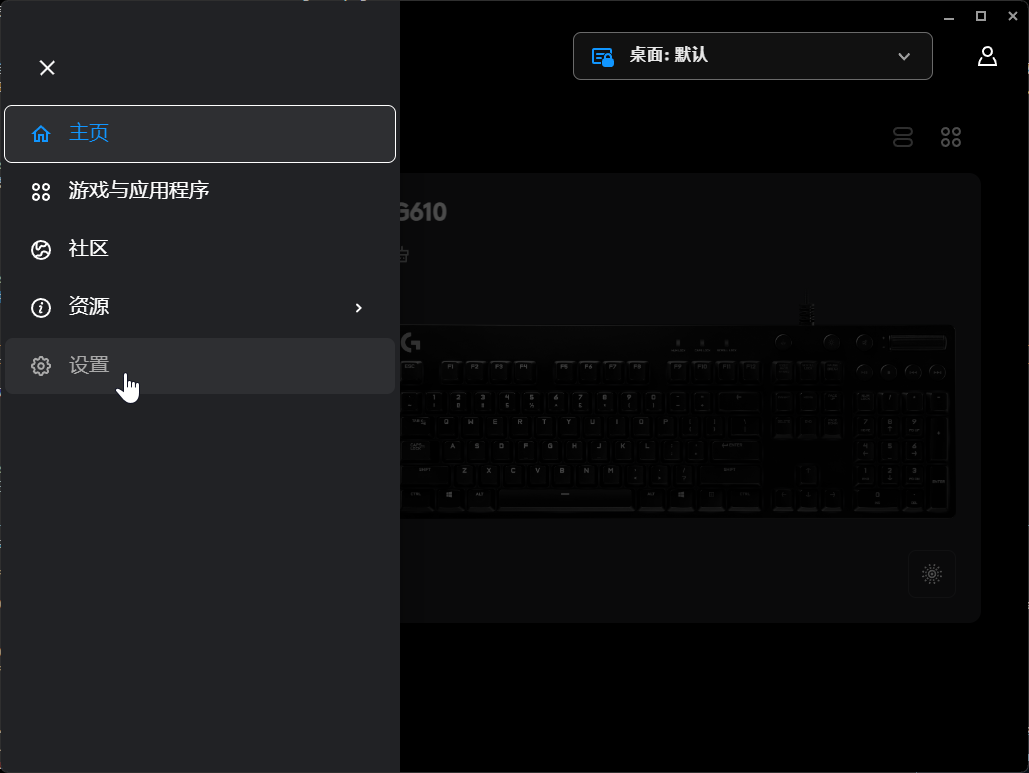
\includegraphics[width=\textwidth]{assets/intro/lghub_setting.png}
    \caption{点击“设置”}
    \label{ch0fig-lghub-setting}
\end{figure}

\begin{figure}[H]
    \Centering
    \parbox[l]{\textwidth}{在设置界面中关闭软件开机自启(图 \ref{ch0fig-disable-login-start}),防止软件以普通权限自启
    (设置软件以管理员权限开机自启的方法可在阅读完本节后参考\nameref{section_skills}章节中的\nameref{subsection-auto-start-lghub-as-admin})。}
    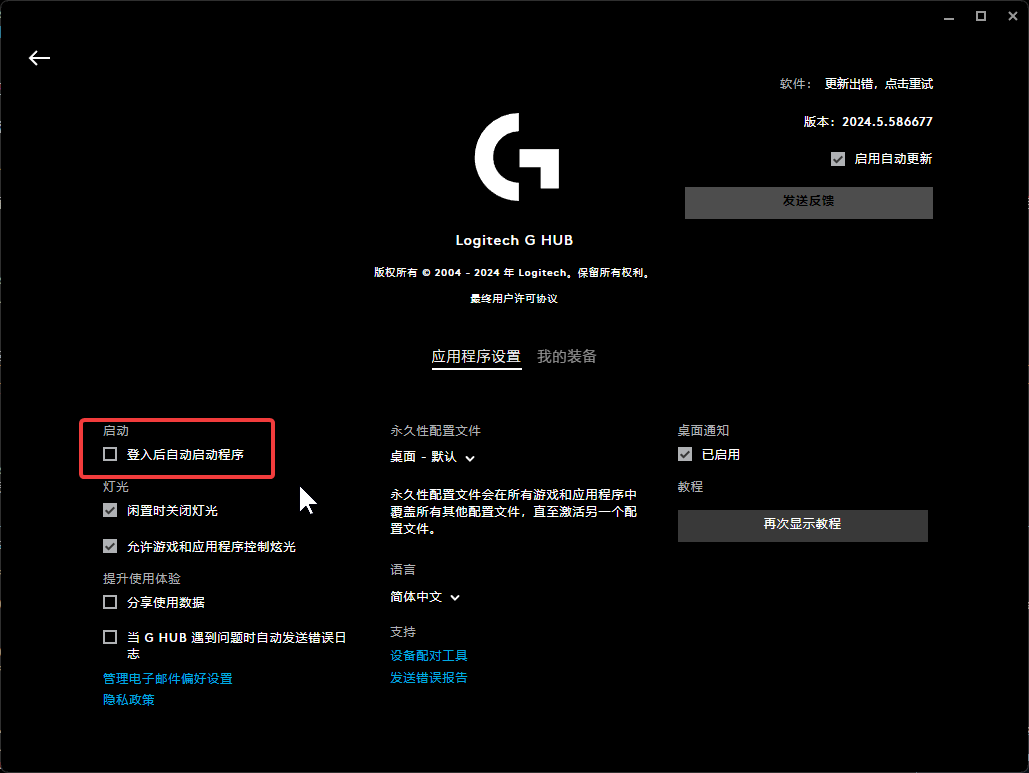
\includegraphics[width=\textwidth]{assets/intro/disable_login_start.png}
    \caption{关闭软件自启}
    \label{ch0fig-disable-login-start}
\end{figure}

\begin{figure}[H]
    \Centering
    \parbox[l]{\textwidth}{返回到主界面,在软件上方下拉框中点击“管理配置文件”(图 \ref{ch0fig-manage-configs})。}
    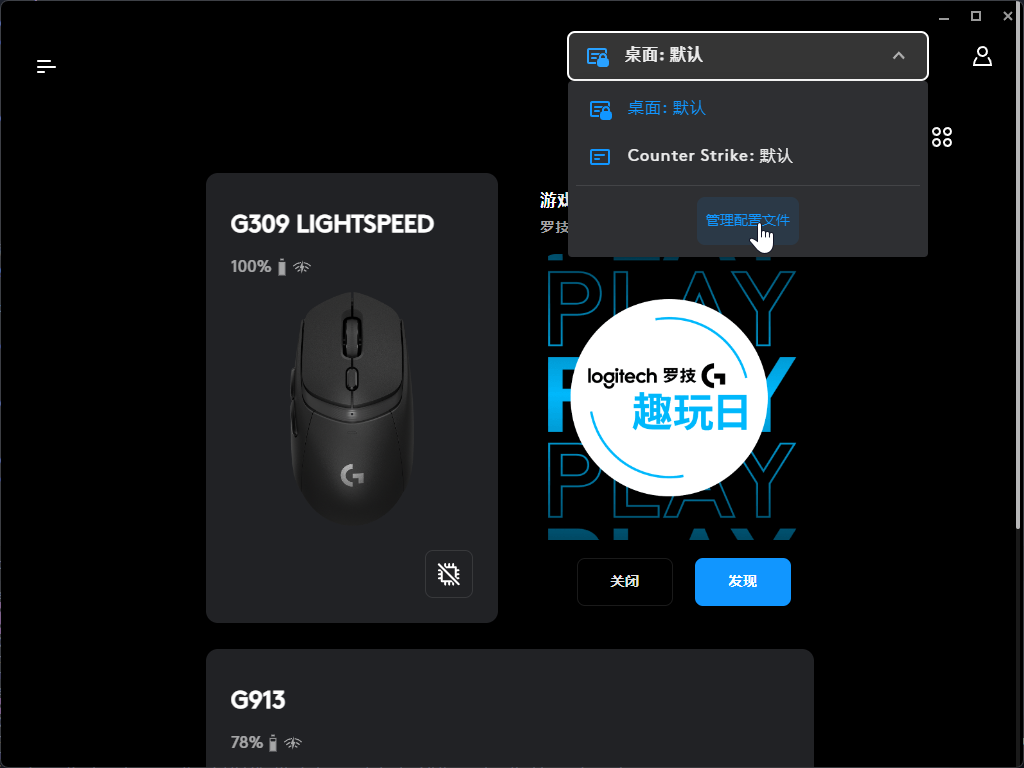
\includegraphics[width=\textwidth]{assets/intro/manage_configs.png}
    \caption{点击“管理配置文件”}
    \label{ch0fig-manage-configs}
\end{figure}

\begin{figure}[H]
    \Centering
    \parbox[l]{\textwidth}{点击其中一个配置项,这里选择默认的“桌面”(图 \ref{ch0fig-script})。}
    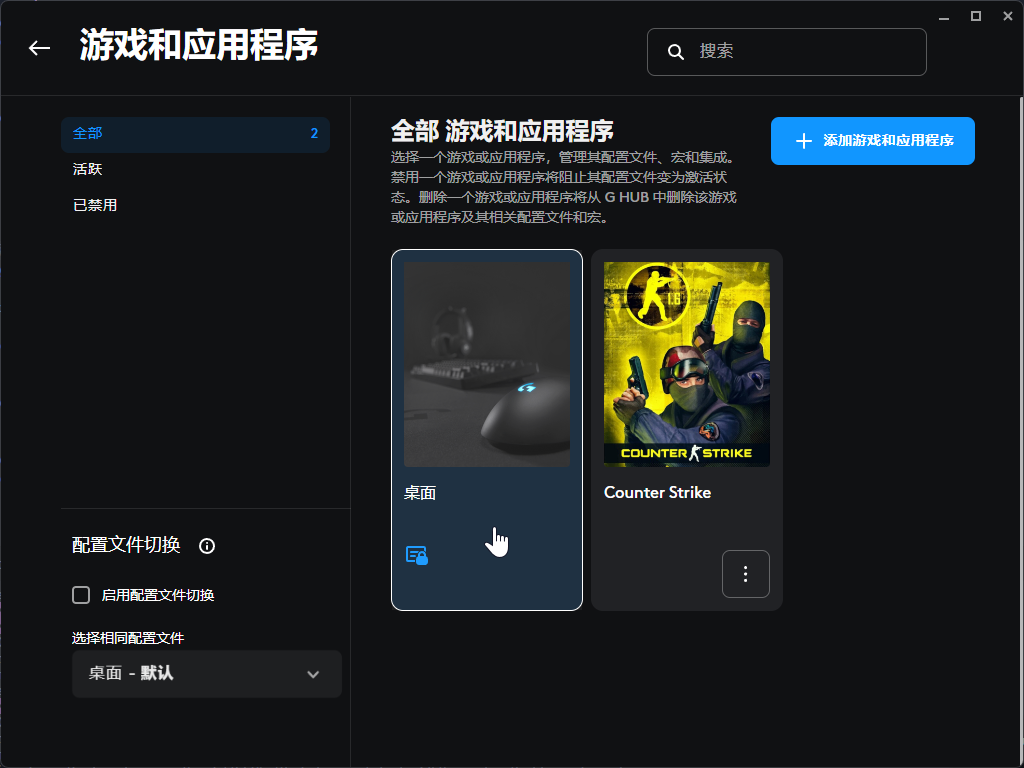
\includegraphics[width=\textwidth]{assets/intro/select_config.png}
    \caption{选择一个配置}
    \label{ch0fig-select-config}
\end{figure}

\begin{figure}[H]
    \Centering
    \parbox[l]{\textwidth}{在下一级界面中点击“创建 LUA 脚本”(图 \ref{ch0fig-script})。}
    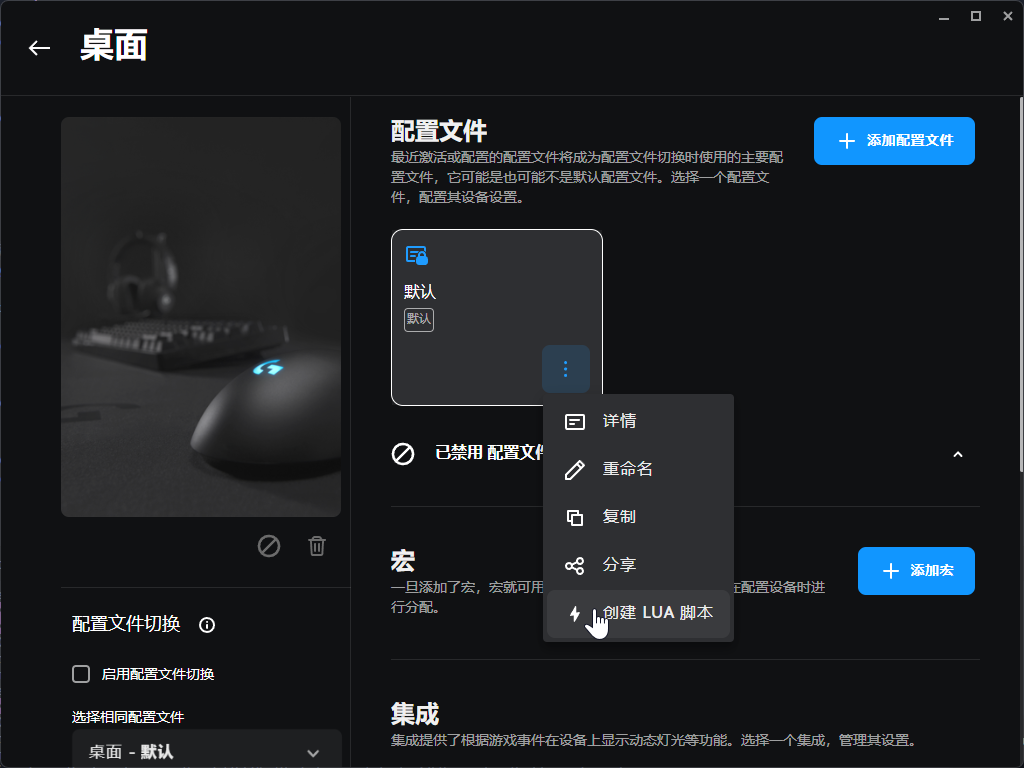
\includegraphics[width=\textwidth]{assets/intro/script.png}
    \caption{点击“编写脚本”}
    \label{ch0fig-script}
\end{figure}

点击“脚本”→“导入”(图 \ref{ch0fig-edit}、\ref{ch0fig-import})。将 Lua 源文件 \lstinline{Executor.lua} 导入软件,点击保存并运行(图 \ref{ch0fig-import-executor-lua}、\ref{ch0fig-save-and-run})。

\begin{figure}[H]
    \Centering
    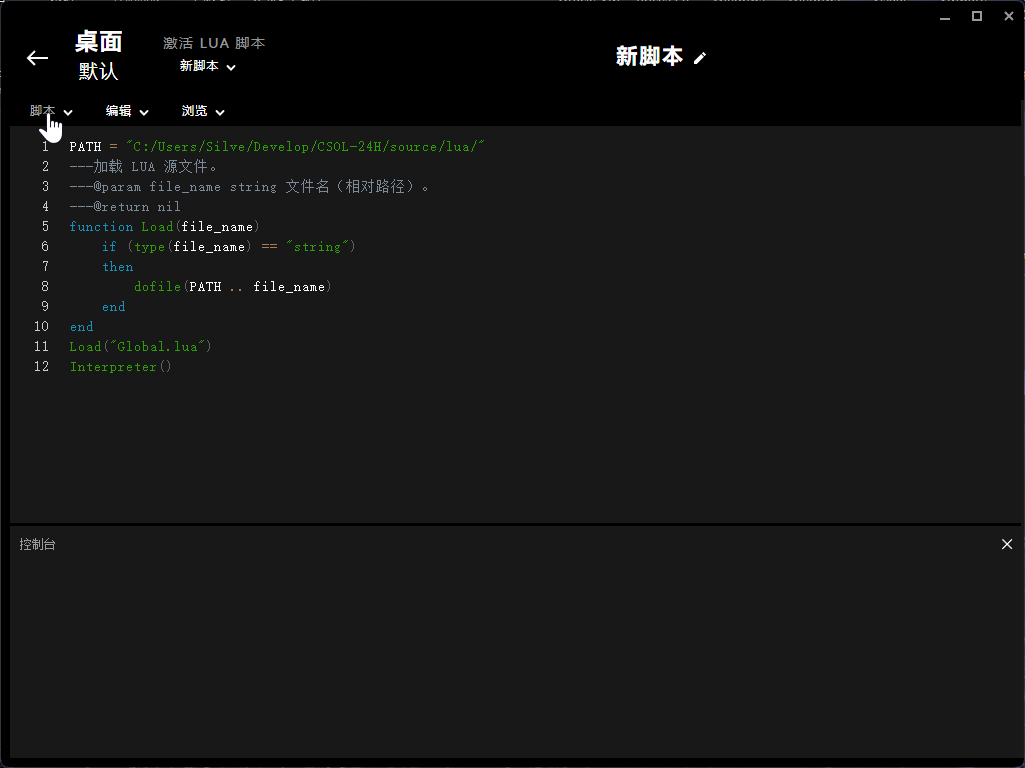
\includegraphics[width=\textwidth]{assets/intro/edit.png}
    \caption{点击“脚本”}
    \label{ch0fig-edit}
\end{figure}

\begin{figure}[H]
    \Centering
    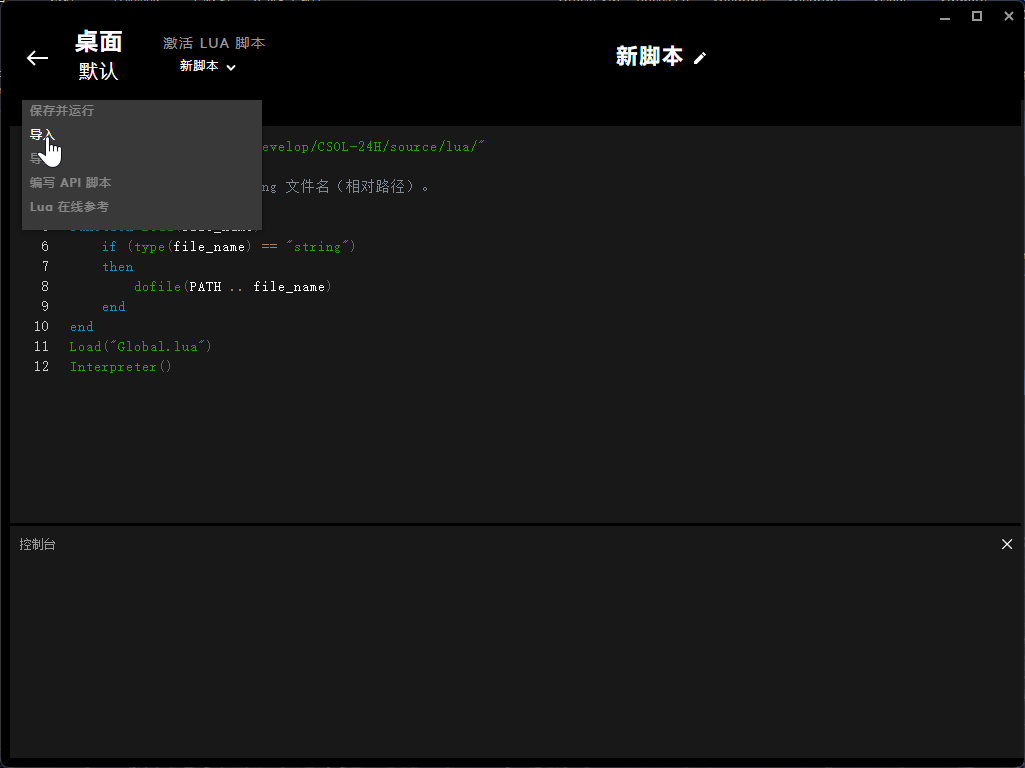
\includegraphics[width=\textwidth]{assets/intro/import.png}
    \caption{点击“导入”}
    \label{ch0fig-import}
\end{figure}

\begin{figure}[H]
    \Centering
    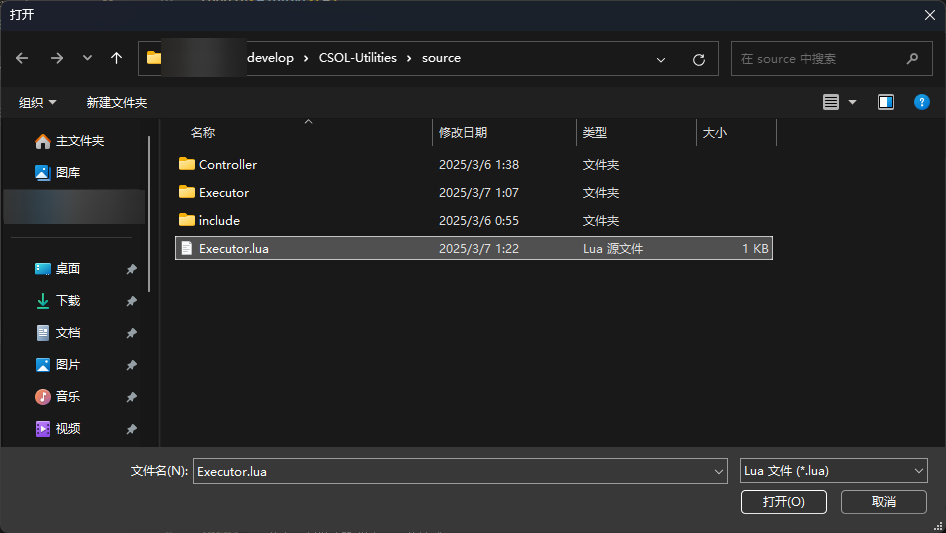
\includegraphics[width=\textwidth]{assets/intro/import_executor.png}
    \caption{选择 \lstinline{Executor.lua} 后导入}
    \label{ch0fig-import-executor-lua}
\end{figure}

\begin{figure}[H]
    \Centering
    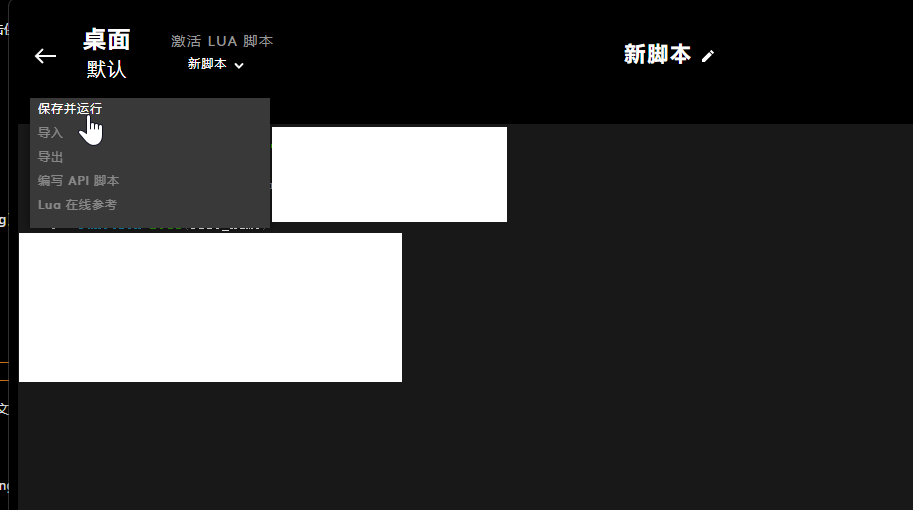
\includegraphics[width=\textwidth]{assets/intro/save_and_run.png}
    \caption{保存并运行}
    \label{ch0fig-save-and-run}
\end{figure}



\begin{figure}[H]
    \Centering
    \parbox[l]{\textwidth}{看到控制台输出下述文字信息(图 \ref{ch0fig-success}),则说明导入成功。}
    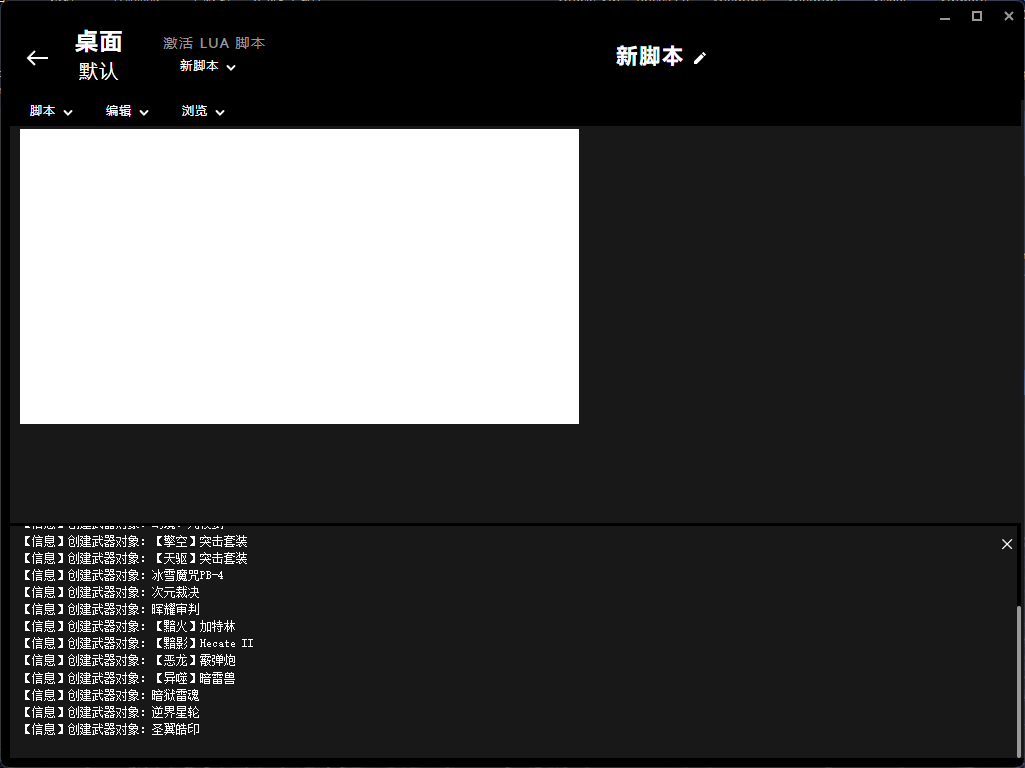
\includegraphics[width=\textwidth]{assets/intro/success.png}
    \caption{保存并运行成功}
    \label{ch0fig-success}
\end{figure}

保存并运行后,罗技软件在下一次启动时会自动加载上述脚本文件,无需再重复上述操作。

\textbf{\color{red}但是,若后续您对 \lstinline{lua} 子目录下的任一个文件进行修改(例如修改配置文件,参见后续章节),则还需要重新在此界面中保存运行以使改动生效。}

\subsection{控制器}

控制器是用于实时向执行器模块下达命令的状态机,模块的运行依赖于控制器向其下达的命令。

\begin{figure}[H]
    \Centering
    \parbox[l]{\textwidth}{双击运行 \lstinline{Controller.cmd}(图 \ref{ch0fig-run-controller}),控制器将在初始化运行环境后启动。}
    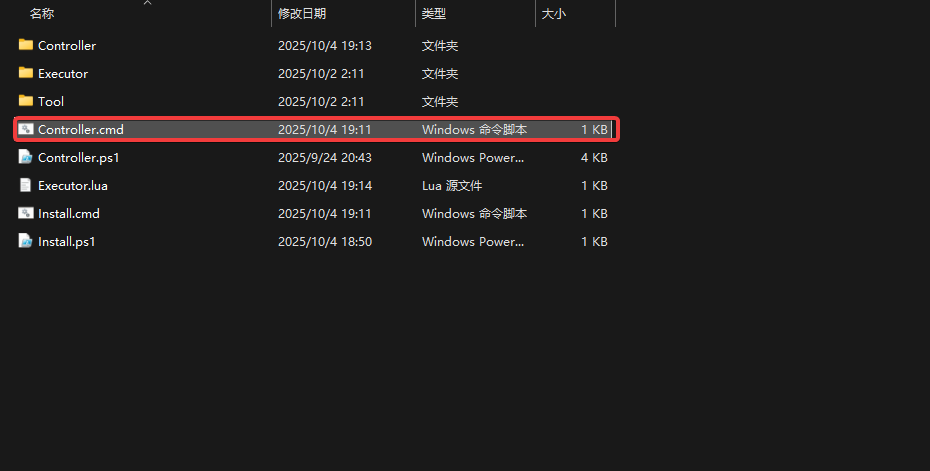
\includegraphics[width=\textwidth]{assets/intro/run_controller.png}
    \caption{运行控制器}
    \label{ch0fig-run-controller}
\end{figure}

启动控制器后,控制器会在系统中注册如下全局热键(在阅读完本节之前请先不要尝试,控制器退出时这些热键会自动注销):

\begin{itemize}
    \item 0 模式:\lstinline{Ctrl} \lstinline{Alt} \lstinline{Shift} \lstinline{0},启动后的默认模式,该模式下不进行任何操作。

    \item 1 模式:\lstinline{Ctrl} \lstinline{Alt} \lstinline{Shift} \lstinline{1},默认挂机模式。

    \item 2 模式:\lstinline{Ctrl} \lstinline{Alt} \lstinline{Shift} \lstinline{2},扩展挂机模式。

    \item 3 模式:\lstinline{Ctrl} \lstinline{Alt} \lstinline{Shift} \lstinline{3},自动合成配件。

    \item 4 模式:\lstinline{Ctrl} \lstinline{Alt} \lstinline{Shift} \lstinline{4},自动重复购买同一件商店物品,可用于批量购买金币道具。

    \item 5 模式:\lstinline{Ctrl} \lstinline{Alt} \lstinline{Shift} \lstinline{5},定位坐标,将结果输出到罗技控制台。
\end{itemize}

控制器有点像汽车上的档位,只是这里的每个档位具有不同功能。

控制器会在 \lstinline{Executor} 目录下创建临时文件,并实时向该临时文件中写入命令,指挥执行器模块执行相应的命令。
每条命令都有一定的有效期(2 秒左右),超过有效期的命令不会被执行。
每条命令执行完毕都需要一定的时间,因此\textbf{\color{red}控制器切换模式不会立即停止当前命令的执行,而是需要等待当前命令执行完毕才会完成模式切换}。

要退出控制器,您可以直接点击右上角的“×”退出。不过,最推荐做法(非强制性)是打开控制器窗口,鼠标点击控制器窗口内任意处激活控制器窗口,然后按下 \lstinline{Ctrl} \lstinline{C} 退出窗口内运行的控制器。当您看到下图的信息,即表示控制器成功退出,然后再点击“×”关闭窗口。
这使得控制器有充足的时间释放资源,然后安全地退出。

\begin{figure}[H]
    \Centering
    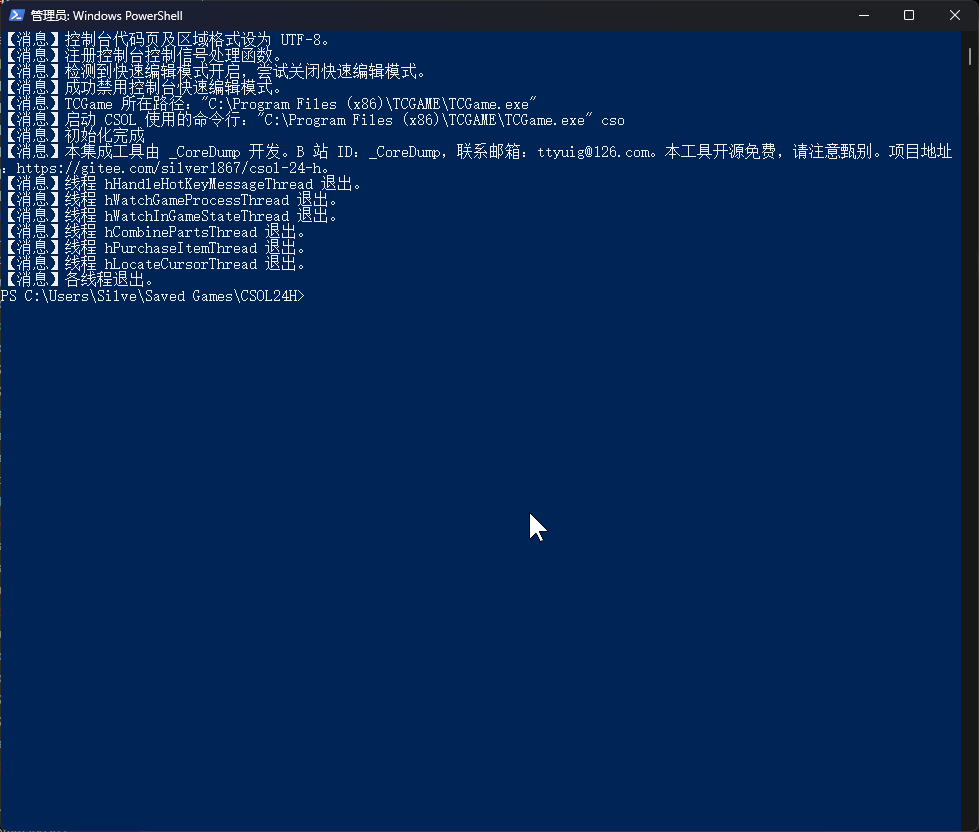
\includegraphics[width=\textwidth]{assets/intro/exit_controller.png}
    \caption{退出控制器的最佳做法}
\end{figure}

v1.3.19 之后,控制器运行于挂机模式(1 号模式或 2 号模式)时,将会终止所有正在运行的 CSOBanner 进程(游戏退出后的广告)。

\subsection{执行器及其即时中断功能}

执行器模块有点像汽车的发动机,它是真正负责执行控制器命令的模块。

上面提到,控制器切换模式后到执行器模块响应模式切换有一定的延迟,在执行器模块执行完当前命令后才会进行模式切换,这会导致您在模式切换成功前键盘鼠标不受控制。
为了使罗技软件能够及时响应您接管键盘鼠标的需要,本集成工具通过在执行器模块中引入了\textbf{即时中断}功能,旨在随时暂停和恢复执行器模块的运行。

\begin{itemize}
\item 暂停:同时按下键盘上的左右 \lstinline{Ctrl} 键(作用类似于踩下离合器空挡)。
\item 恢复:同时按下键盘上的左右 \lstinline{Alt} 键(作用类似于抬起离合器传动)。
\end{itemize}

例如,\textbf{\color{red}若不慎错误地按下前面提及的功能热键(挂错档),导致鼠标键盘不受控制,可以同时按下键盘上的左 \lstinline{Ctrl} 和右 \lstinline{Ctrl} 紧急暂停(踩下离合器),罗技软件会在 10 毫秒内快速响应此中断信号。
紧急暂停后,罗技软件仍会接收来自控制器的命令,但不会发出任何键鼠操作(发动机空转),直至同时按下键盘上的左 \lstinline{Alt} 和右 \lstinline{Alt} 恢复(抬起离合器)。}

相应地,您可以在罗技软件控制台中看到相应的提示信息。

\begin{figure}[H]
    \Centering
    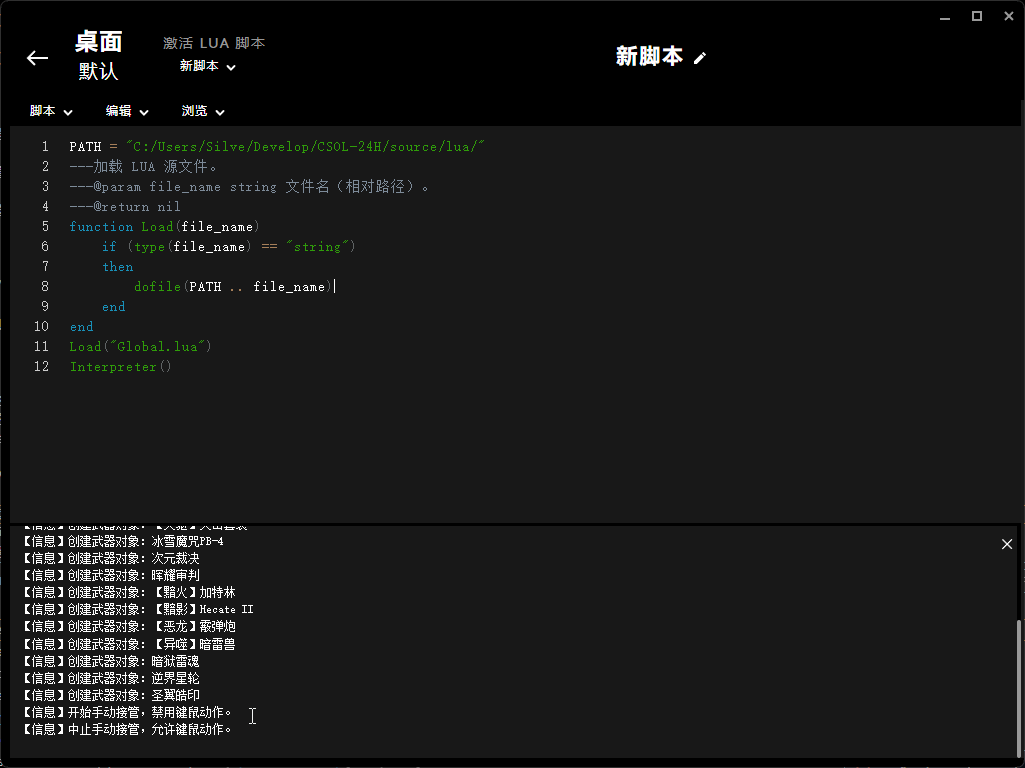
\includegraphics[width=\textwidth]{assets/intro/interrupt.png}
    \caption{即时中断功能提示信息}
\end{figure}

\textbf{\color{red}执行器模块在执行过程中会进行按键操作(如模拟按下数字键),这会对模式切换造成影响,导致您切换到错误的模式。
因此,当需要从一个模式切换到另一个模式时,建议先暂停执行器模块,然后再按相应热键进行模式切换,切换完成后再恢复执行器模块执行。
这个过程有点像您在开车换档时需要先踩下离合器空挡(暂停),换档完成后(切换模式)再抬起离合器(恢复)。}

\textbf{\color{red}需要注意,上述中断功能(离合器)独立于控制器(档位)。执行器模块暂停后(踩下离合器),控制器仍然会持续向罗技软件下达命令(档位没有改变),只是罗技软件并不会真正执行这些命令(发动机空转)。若要取消当前控制器启用的模式,请按热键将控制器切换回 0 模式(挂空挡)。}

\subsection{配置文件}

\textbf{\color{red}\lstinline{lua} 目录下的 \lstinline{Setting.lua} 及 \lstinline{WeaponList.lua} 是根据用户自身情况自行定义的配置文件。有关配置文件的使用方法参见后续章节。
按照本文档介绍的方式配置完毕且能够正常使用后,您应当妥善保管。后续版本更新不会对这两个配置文件内容作出较大的变动。当您修改配置文件内容后,必须在罗技软件中重新导入并保存运行。}

\subsection{关于编程接口}

对于具有一定编程经验的用户,阅读完本手册内容后可以访问 \href{https://blog.macrohard.fun/CSOL-Utilities/}{CSOL 集成工具开发者文档} 了解更多定制化使用方法。
